% First LaTeX draft of the time-aware fusion paper (from the shared draft doc, 2026-10-17).
% Layout: IEEE two-column conference format on A4 as a page-count proxy.
% Target venue: RSS 2027 Stage 1 (due 2026-12-04). Before submission: port to the RSS
% template, anonymize, no repository links, no page numbers, compile with pdflatex.
\documentclass[conference,a4paper]{IEEEtran}

\usepackage[T1]{fontenc}
\usepackage{amsmath,amssymb}
\usepackage{booktabs}
\usepackage{xcolor}
\usepackage{tikz}
\usetikzlibrary{arrows.meta,positioning}
\usepackage{pgfplots}
\pgfplotsset{compat=1.17}
\usepackage{cite}
\usepackage[hidelinks]{hyperref}

\newcommand{\pending}[1]{\textcolor{red}{[PENDING: #1]}}
\newcommand{\todo}[1]{\textcolor{orange}{[TODO: #1]}}

\begin{document}

\title{Time Is the Baseline to Beat: Calibrated Fusion of\\
Policy-Internal Scores and Elapsed Time for VLA Failure Detection}

\author{\IEEEauthorblockN{Felix Doublet}
\IEEEauthorblockA{Shinoda Lab \todo{affiliation and co-authors}}}

\maketitle

\begin{abstract}
Runtime failure detectors for vision-language-action (VLA) policies are rarely compared
against elapsed time. Failed rollouts tend to run until the task timeout, so a
task-conditioned time-risk detector that sees no policy features catches 63\% of failures
at a 5\% false-positive rate (FPR) on 38 RoboCasa365 tasks with Xiaomi-Robotics-1, more
than the SAFE failure predictor alone (57\%). We propose time-aware fusion: alarm when
either a policy-internal score or the time risk crosses its threshold, with both
thresholds calibrated jointly on a separate cohort and evaluated once on a disjoint
prospective cohort. \pending{one sentence: preregistered confirmatory result on 760 fresh
rollouts.} On the prospective cohort used to develop the design, fusion raised recall to
0.955 at 0.058 FPR. Four success-only anomaly scores fused the same way reached
0.905--0.947, with no significant difference from fused SAFE, so the gain comes from the
fusion rather than from a particular learned score. The gain is not an artifact of failed
rollouts running longer: random noise fused with time under the same calibration recovers
only the time-only recall (0.635 on average over 50 draws). Alarms remain late: no detector
catches more than 3\% of failures within the first quarter of the task horizon, and fused
alarms fire a median of 12 policy inferences before the rollout ends.
\end{abstract}

\section{Introduction}

A failure detector earns its place only if it beats what a robot already knows for free:
how long the current attempt has been running. Generalist VLA policies still fail often on
household tasks, and a deployed system needs an online signal that a rollout is going
wrong. Recent detectors read the policy's internal features and learn to predict eventual
failure~\cite{gu2025safe}. Others score how unusual those features are relative to
successful rollouts~\cite{xu2025faildetect,lee2018mahalanobis,sun2022knn}.

These detectors are usually evaluated on completed rollouts, where a strong shortcut hides.
Successful rollouts stop at first success, while failures typically run to the timeout. In
our data, completed-rollout duration alone reaches ROC-AUC 0.80 on a held-out test of 76
rollouts, against 0.53 for the raw SAFE score and 0.69 after per-task normalization. SAFE
avoids this shortcut by truncating rollouts to equal length~\cite{gu2025safe}, but a
deployed detector cannot truncate. A causal version of this shortcut is legitimate at deployment: the probability that
the task will fail, given that it is still running at step $t$. Any learned detector must
therefore beat this elapsed-time risk at the same false-positive budget, not just chance.

We make this comparison under a strict protocol. Detectors are developed on one cohort,
their thresholds are frozen on a separate calibration cohort at a 5\% event-level FPR, and
they are then evaluated once on a disjoint prospective cohort. We write down how each
outcome will be interpreted before opening each new result. Our contributions are:
\begin{enumerate}
  \item \textbf{Elapsed time as the reference.} A task-conditioned time-risk detector
  catches 63.2\% of failures at 4.7\% FPR on 760 prospective rollouts of
  Xiaomi-Robotics-1 on 38 RoboCasa365 tasks. Policy-feature scores used alone do no
  better at the same budget.
  \item \textbf{Time-aware fusion.} Alarming when either a policy-internal score or the
  time risk crosses a jointly calibrated threshold raises recall to 95.5\% at 5.8\% FPR.
  \pending{confirmatory result on a fresh cohort.}
  \item \textbf{The fusion matters more than the representation.} SAFE, Mahalanobis, kNN,
  PCA-KMeans and RND scores all reach 90--95\% recall once fused with time. Their
  differences from fused SAFE are not significant, although the data cannot exclude
  differences of up to 0.15 recall. Random noise or label-free resampled SAFE scores fused
the same way add at most about 3 points over time alone, so the gain needs a policy-internal
signal, not just a score that grows with rollout length.
\end{enumerate}
Our original, preregistered design restricted the policy score to the first quarter of
the rollout and gained only 3.7 points of recall over time alone; we report it as such.

\section{Related Work}

\textbf{Failure detection from policy internals.} SAFE trains a small MLP or LSTM on a
VLA's internal features to predict eventual failure, and thresholds it with functional
conformal prediction~\cite{gu2025safe}; we reuse its implementation. SAFE notes that a
detector could simply count elapsed time and removes this shortcut by truncating rollouts to
equal length. We instead keep elapsed time, as a calibrated, deployable baseline and as a
signal to fuse. In machine-learning terms, duration is a shortcut
feature~\cite{geirhos2020shortcut}, but at deployment its causal form is legitimate
evidence. Recent probes improve labels, robustness or
calibration~\cite{park2026hideseek,ma2026failurespot,rajaprakash2026safecast}, and VLA-Scope
adds execution-progress features to a learned predictor~\cite{zhu2026vlascope}. None compares
against elapsed time alone.

\textbf{Detectors without failure data.} FAIL-Detect scores policy inputs and outputs
against successful rollouts only~\cite{xu2025faildetect}. FIPER alarms when an RND score on
policy embeddings and an action-chunk entropy \emph{both} exceed conformal
thresholds~\cite{romer2025fiper}. Requiring both signals suits FIPER's aim of suppressing
false alarms. Our fusion instead fires when \emph{either} signal crosses, so that each can
catch failures the other misses, and the joint calibration keeps the combined FPR within
budget. On our data, AND-fusion calibrated the same way reached higher test recall
(1.000) but overshot the FPR budget further (0.089, Wilson 95\% upper bound 0.122).

\textbf{Consistency and VLM monitors.} STAC~\cite{agia2024sentinel},
VLA-FAIL~\cite{seligmann2026vlafail} and ActProbe~\cite{huang2026actprobe} compare the
overlapping parts of consecutive action chunks. Xiaomi-Robotics-1 executes each 16-step chunk
in full, so this signal is undefined for our policy. Language and vision-language monitors judge
task progress, detect anomalies or explain failures from
frames~\cite{agia2024sentinel,duan2025aha,liu2023reflect,sinha2024realtime,zhou2025codeasmonitor}
and are complementary to the time signal.

\textbf{Time-to-event modelling.} Our time risk is a per-task survival-style estimate of
the probability of failure given that a rollout is still running, in the tradition of
Kaplan--Meier and hazard models~\cite{kaplan1958,cox1972}. Deciding when to stop observing
a sequence and declare its class is studied as early time-series
classification~\cite{xing2012early}; our recall-versus-horizon analysis is its
accuracy-earliness trade-off.

\textbf{OOD scores and calibration.} We use SAFE's embedding baselines: Mahalanobis
distance~\cite{lee2018mahalanobis}, $k$-nearest-neighbour distance~\cite{sun2022knn}, PCA
plus $k$-means distance, and random network distillation~\cite{burda2019rnd}, all fitted on
successful rollouts. Conformal thresholds give finite-sample false-positive control under
exchangeability~\cite{angelopoulos2021gentle}. Most prior evaluations report ROC-AUC and one
operating point on the test pool. We instead freeze every threshold on a separate calibration
cohort and compare detectors at a matched event-level FPR on a disjoint prospective cohort.

\section{Problem Setting and Metrics}

A detector watches one rollout of a known task $k$ and decides online, at each policy
inference $t = 1, 2, \dots$ (one inference per 16-step action chunk), whether to raise an
alarm. The task horizon $H_k$ is the length, in inferences, of the longest failed
development rollout of task $k$, a proxy for the task timeout. Its score at $t$ may use only what is
available by $t$: the policy features so far, the inference index and the task identity.
It may not use the rollout's final length, future features, or subtask annotations. The
first threshold crossing is the alarm; the detector never changes the policy's actions.

Failure is the positive class. A failed rollout is detected if any alarm fires before it
ends; a successful rollout with any alarm is a false positive. We report event-level TPR
and FPR, balanced accuracy (BA), the \emph{miss-adjusted detection fraction}---the
first-alarm time as a fraction of the task horizon $H_k$, averaged over all failures with a
missed failure counted as 1.0 (lower is earlier)---and recall at 10\%, 25\% and 50\% of
$H_k$. All detectors are compared at operating points fixed on the calibration cohort under
FPR $\le 0.05$. Confidence intervals come from a paired bootstrap that resamples tasks, then
rollouts within each task (2,000 replicates).

\section{Method}

\begin{figure}[t]
\centering
\resizebox{\columnwidth}{!}{%
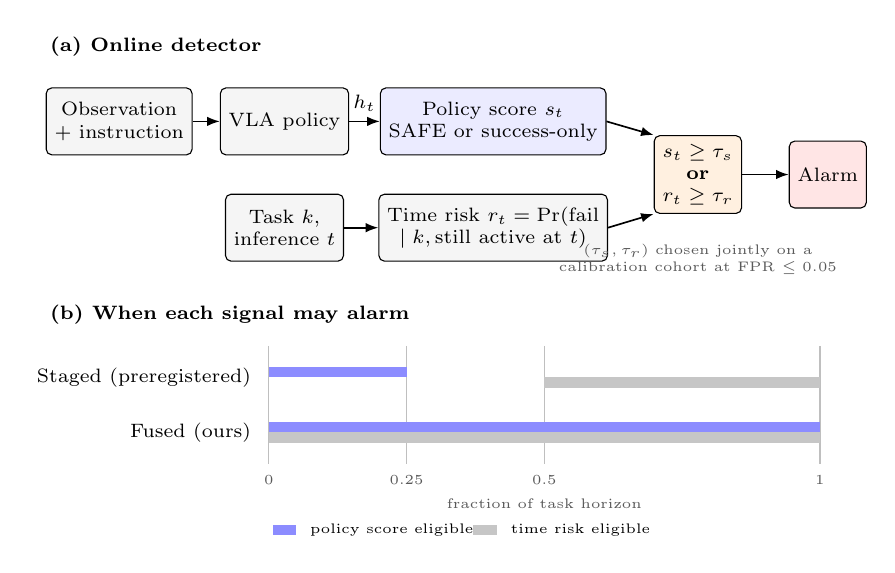
\begin{tikzpicture}[font=\scriptsize,
  box/.style={draw, rounded corners=2pt, align=center, minimum height=0.85cm, inner sep=3pt},
  arr/.style={-{Latex[length=1.6mm]}, semithick}]
  % (a) pipeline
  \node[anchor=west,font=\scriptsize\bfseries] at (-1.0,0.95) {(a) Online detector};
  \node[box, fill=gray!8] (obs) at (0,0) {Observation\\+ instruction};
  \node[box, fill=gray!8] (vla) at (2.1,0) {VLA policy};
  \node[box, fill=blue!8] (score) at (4.75,0) {Policy score $s_t$\\SAFE or success-only};
  \node[box, fill=gray!8] (task) at (2.1,-1.35) {Task $k$,\\inference $t$};
  \node[box, fill=gray!8] (time) at (4.75,-1.35) {Time risk $r_t = \Pr(\text{fail}$\\$\mid k, \text{still active at } t)$};
  \node[box, fill=orange!12] (or) at (7.35,-0.675) {$s_t \ge \tau_s$\\\textbf{or}\\$r_t \ge \tau_r$};
  \node[box, fill=red!10] (alarm) at (9.0,-0.675) {Alarm};
  \draw[arr] (obs) -- (vla);
  \draw[arr] (vla) -- node[above, font=\scriptsize] {$h_t$} (score);
  \draw[arr] (task) -- (time);
  \draw[arr] (score.east) -- (or.north west);
  \draw[arr] (time.east) -- (or.south west);
  \draw[arr] (or) -- (alarm);
  \node[align=center, font=\tiny, text=gray!70!black] at (7.35,-1.75)
    {$(\tau_s,\tau_r)$ chosen jointly on a\\calibration cohort at FPR $\le 0.05$};
  % (b) eligibility windows
  \node[anchor=west,font=\scriptsize\bfseries] at (-1.0,-2.45) {(b) When each signal may alarm};
  \def\xa{1.9} \def\xb{8.9}
  \foreach \f/\l in {0/0, 0.25/0.25, 0.5/0.5, 1/1}{
    \draw[gray!50] ({\xa+\f*(\xb-\xa)},-2.85) -- ({\xa+\f*(\xb-\xa)},-4.35);
    \node[gray!70!black, font=\tiny] at ({\xa+\f*(\xb-\xa)},-4.55) {\l};
  }
  \node[gray!70!black, font=\tiny] at ({(\xa+\xb)/2},-4.85) {fraction of task horizon};
  \node[anchor=east] at (\xa-0.1,-3.25) {Staged (preregistered)};
  \fill[blue!45] (\xa,-3.12) rectangle ({\xa+0.25*(\xb-\xa)},-3.25);
  \fill[gray!45] ({\xa+0.5*(\xb-\xa)},-3.25) rectangle (\xb,-3.38);
  \node[anchor=east] at (\xa-0.1,-3.95) {Fused (ours)};
  \fill[blue!45] (\xa,-3.82) rectangle (\xb,-3.95);
  \fill[gray!45] (\xa,-3.95) rectangle (\xb,-4.08);
  \fill[blue!45] (\xa+0.05,-5.25) rectangle (\xa+0.35,-5.12);
  \node[anchor=west, font=\tiny] at (\xa+0.4,-5.185) {policy score eligible};
  \fill[gray!45] (\xa+2.6,-5.25) rectangle (\xa+2.9,-5.12);
  \node[anchor=west, font=\tiny] at (\xa+2.95,-5.185) {time risk eligible};
\end{tikzpicture}}
\caption{Time-aware fusion. (a) At each policy inference, a policy-internal score and a
task-conditioned elapsed-time risk are compared with two thresholds; the first crossing of
either raises the alarm. Both thresholds are set together on a separate calibration cohort.
(b) The preregistered staged design let the policy score alarm only in the first quarter of
the rollout and time only after half; fusion lets both alarm throughout.}
\label{fig:method}
\end{figure}

Time-aware fusion (Fig.~\ref{fig:method}) combines two causal scores, each with its own
threshold, and alarms as soon as either crosses. Both thresholds are chosen together on a calibration cohort so that
the combined detector meets the FPR budget.

\subsection{Policy-internal score}

\textbf{SAFE.} At each inference we take the final-layer action-token hidden state of the
policy's flow-matching DiT, just before its action output layer (1,024 dimensions, last
flow step, last action position). The official SAFE MLP maps it to a failure score
$u^{(j)}_t$ for each of three training seeds $j$. With per-task location $m^{(j)}_k$ and
scale $\sigma^{(j)}_k$ (median, and the larger of the scaled MAD and the standard deviation,
of each development rollout's maximum score), the policy score is
\begin{equation}
  s_t = \frac{1}{3}\sum_{j=1}^{3} \frac{\max_{t' \le t} u^{(j)}_{t'} - m^{(j)}_k}{\sigma^{(j)}_k}.
\end{equation}
The running maximum does not change when a threshold is first crossed; it makes $s_t$
monotone. We use the MLP head because it ranked failures best after task normalization on
held-out development data (ROC-AUC 0.69 against 0.65 for the LSTM).

\textbf{Success-only scores.} Mahalanobis, cosine kNN, PCA-KMeans and feature-space RND
are fitted on successful development rollouts only, so they need no failure labels. Each
produces a per-inference distance, aggregated causally (development selected a cumulative
sum for all four) and normalized per task. Hyperparameters were chosen on held-out
development data by early at-risk ROC-AUC.

\subsection{Elapsed-time risk}

The time risk is the probability that a still-running rollout of task $k$ will fail:
\begin{equation}
  r_t = \Pr(\text{failure} \mid \text{task } k,\ \text{rollout still active at inference } t).
\end{equation}
Among the development rollouts of task $k$ still active at $t$, let $n_t$ be their number
and $f_t$ the number that fail. We take the smoothed ratio $(f_t + 0.5)/(n_t + 1)$ for
$t = 1, \dots, H_k$ and fit an increasing isotonic regression in $t/H_k$, weighted by
$n_t$. This is a survival-style estimate with no policy features. It is causal, because it
uses only whether the rollout is still running. It needs failed development rollouts, but
only to estimate this curve.

\subsection{Calibrated fusion}

The fused detector alarms at the first inference where either score crosses its threshold:
\begin{equation}
  T_{\text{alarm}} = \min \{\, t : s_t \ge \tau_s \ \text{or}\ r_t \ge \tau_r \,\}.
\end{equation}
The pair $(\tau_s, \tau_r)$ is searched jointly on the calibration cohort over every pair
of per-rollout maxima observed on the 228 calibration rollouts. Among pairs with event-level FPR
$\le 0.05$, we keep the one with the highest recall, then the earliest miss-adjusted
detection, then the more conservative thresholds. A successful rollout counts as a false
positive if either score alarms at any time.

\subsection{Staged variant (preregistered)}

Our original design restricted the policy score to the start of the rollout, where elapsed
time cannot separate outcomes, and used time as a late fallback: the policy score may alarm
only while $t \le 0.25 H_k$, and the time risk only from $t \ge 0.5 H_k$. Thresholds are
searched the same way. We froze this variant before the prospective test and report it as
preregistered.

\section{Experimental Setup}

\begin{table*}[t]
\centering
\caption{Prospective test (380 successes, 380 failures), thresholds frozen on calibration
at FPR $\le 0.05$. BA = balanced accuracy; adj = miss-adjusted detection fraction (lower is
earlier). $\Delta$ = paired recall difference with task-then-rollout bootstrap 95\% CI.
Fused rows were defined after this cohort was opened for the staged design. $^\ast$One of
50 random draws; mean recall over draws 0.635 (noise) and 0.650 (resampled).}
\label{tab:main}
\footnotesize
\setlength{\tabcolsep}{3.2pt}
\begin{tabular}{@{}lcccccc@{}}
\toprule
Detector & Recall & FPR & BA & adj & $\Delta$ recall vs.\ time & $\Delta$ recall vs.\ fused SAFE \\
\midrule
Time only & 0.632 & 0.047 & 0.792 & 0.880 & -- & $-0.324$ [$-0.469$, $-0.178$] \\
SAFE only & 0.566 & 0.039 & 0.763 & 0.810 & $-0.065$ [$-0.354$, $+0.215$] & $-0.389$ [$-0.568$, $-0.218$] \\
Success-only scores alone (4) & .582--.666 & .055--.068 & .763--.799 & .782--.818 & $-0.050$ to $+0.035$, CIs span 0 & -- \\
Staged SAFE + time (preregistered) & 0.668 & 0.050 & 0.809 & 0.854 & $+0.037$ [$+0.000$, $+0.090$] & $-0.287$ [$-0.426$, $-0.156$] \\
Staged kNN + time & 0.666 & 0.061 & 0.803 & 0.857 & $+0.035$ [$+0.000$, $+0.097$] & $-0.289$ [$-0.431$, $-0.157$] \\
Staged Mahal., PCA-KM, RND + time & 0.639 & .045--.050 & .795--.797 & .876--.877 & $+0.008$ [$+0.000$, $\le$$+0.026$] & -- \\
\midrule
Fused SAFE + time & 0.955 & 0.058 & 0.949 & 0.816 & $+0.324$ [$+0.178$, $+0.469$] & -- \\
Fused kNN + time & 0.947 & 0.068 & 0.939 & 0.769 & $+0.316$ [$+0.142$, $+0.495$] & $-0.008$ [$-0.093$, $+0.072$] \\
Fused Mahalanobis + time & 0.939 & 0.068 & 0.936 & 0.783 & $+0.308$ [$+0.133$, $+0.484$] & $-0.016$ [$-0.097$, $+0.065$] \\
Fused PCA-KMeans + time & 0.924 & 0.061 & 0.932 & 0.785 & $+0.293$ [$+0.105$, $+0.479$] & $-0.031$ [$-0.130$, $+0.061$] \\
Fused RND + time & 0.905 & 0.063 & 0.921 & 0.794 & $+0.275$ [$+0.082$, $+0.469$] & $-0.049$ [$-0.153$, $+0.050$] \\
\midrule
Fused noise + time (null)$^\ast$ & 0.632 & 0.047 & 0.792 & 0.878 & $+0.000$ [$+0.000$, $+0.000$] & $-0.324$ [$-0.469$, $-0.178$] \\
Fused resampled SAFE + time (null)$^\ast$ & 0.655 & 0.063 & 0.796 & 0.869 & $+0.023$ [$+0.000$, $+0.081$] & $-0.301$ [$-0.446$, $-0.162$] \\
AND-fused SAFE + time & 1.000 & 0.089 & 0.955 & 0.798 & $+0.369$ [$+0.220$, $+0.522$] & $+0.045$ [$+0.005$, $+0.104$] \\
\bottomrule
\end{tabular}
\end{table*}


\textbf{Policy and tasks.} We use the released Xiaomi-Robotics-1 RoboCasa365
checkpoint~\cite{xiaomi2026robotics} at a pinned revision. It predicts 16-step action chunks
with a five-step flow-matching DiT and executes each chunk in full. We take the 39 official
RoboCasa365 tasks~\cite{nasiriany2024robocasa,robocasa365} whose published success count
lies between 5 and 45 out of 50, and drop one with too few failures, leaving 38 tasks
(10 atomic, 28 composite).



\textbf{Cohorts.} We use four disjoint cohorts, each for one purpose
(Table~\ref{tab:cohorts}). Each evaluation cohort is collected from fresh environment
seeds until every task has a fixed quota of successes and failures. The primary cohort
takes the first rollouts of each class per task in seed order. Rollouts past the quota
form a secondary all-retained cohort. No two cohorts share a seed or reset.

\begin{table}[t]
\centering
\caption{Cohorts. S/F = successes/failures. The primary cohort takes the first $q$
rollouts of each class per task; ``retained'' adds every rollout collected past the quota.}
\label{tab:cohorts}
\footnotesize
\begin{tabular}{@{}llrr@{}}
\toprule
Cohort & Used to & Primary (S/F, $q$) & Retained \\
\midrule
Development & fit SAFE, scores, time & 1,824 & -- \\
Calibration & set thresholds & 228 (114/114, 3) & 454 \\
Prospective test & evaluate once & 760 (380/380, 10) & 1,643 \\
Confirmatory & preregistered test & 760 (380/380, 10) & pending \\
\bottomrule
\end{tabular}
\end{table}

\textbf{Frozen protocol.} The staged detector, all SAFE checkpoints, normalization and time
curves were frozen before the prospective test was collected. The baselines and fused
detectors were added later and evaluated once on the same opened cohort, with thresholds
taken from calibration only. Each run first had to reproduce the frozen results and
thresholds exactly and verify the checksums of the frozen inputs. Before each new
evaluation we wrote down how we would interpret every outcome, including the rule for
crediting SAFE specifically. These plans, and the confirmatory preregistration, are
timestamped commits in our repository, to be released with the paper.

\textbf{Detectors compared.} Time only; SAFE only; staged SAFE + time (preregistered); fused
SAFE + time; and each success-only score alone, staged with time, and fused with time.
Two null scores test whether fusion only exploits longer failed rollouts, which give any
score more chances to cross. \emph{Noise} is the running maximum of i.i.d.\ Gaussian draws,
one per inference. \emph{Resampled SAFE} draws each inference's raw SAFE scores i.i.d.\ from
all inferences of the same task in the same cohort, ignoring outcomes, and passes them
through the frozen SAFE normalization. Each null is fused with time and calibrated exactly
like fused SAFE, over 50 random draws. Finally, AND-fused SAFE + time alarms once both
scores have crossed, with its own jointly calibrated thresholds. These controls were run
after the review of this draft, on the same opened cohorts.

\section{Results}

On the 760-rollout prospective test, every policy-internal score fused with elapsed time
detects 90--96\% of failures at about 6\% FPR, against 63\% for time alone
(Table~\ref{tab:main}, Fig.~\ref{fig:horizon}).

\begin{figure}[t]
\centering
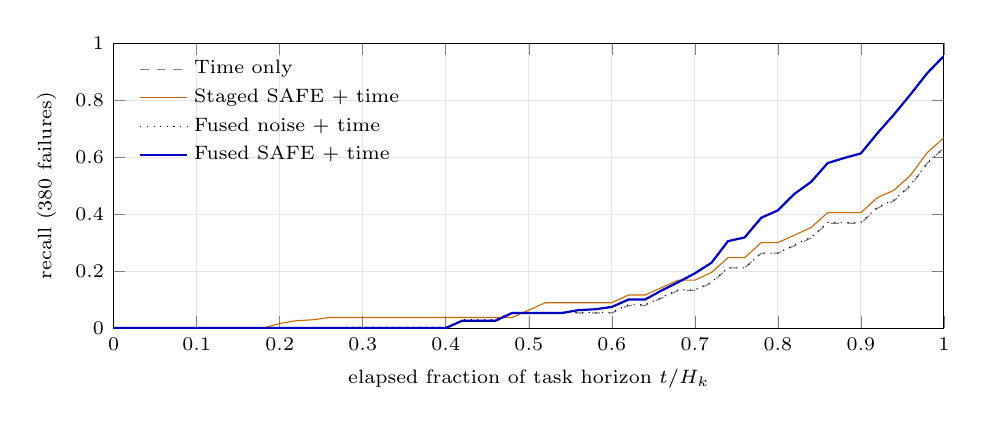
\begin{tikzpicture}
\begin{axis}[width=\columnwidth, height=5.2cm, xmin=0, xmax=1, ymin=0, ymax=1,
  xlabel={elapsed fraction of task horizon $t/H_k$}, ylabel={recall (380 failures)},
  label style={font=\scriptsize}, tick label style={font=\scriptsize},
  legend style={font=\scriptsize, at={(0.02,0.98)}, anchor=north west, draw=none, fill=none},
  legend cell align=left, grid=major, grid style={gray!20}]
\addplot[gray, dashed] coordinates {(0.00,0.000) (0.02,0.000) (0.04,0.000) (0.06,0.000) (0.08,0.000) (0.10,0.000) (0.12,0.000) (0.14,0.000) (0.16,0.000) (0.18,0.000) (0.20,0.000) (0.22,0.000) (0.24,0.000) (0.26,0.000) (0.28,0.000) (0.30,0.000) (0.32,0.000) (0.34,0.000) (0.36,0.000) (0.38,0.000) (0.40,0.000) (0.42,0.026) (0.44,0.026) (0.46,0.026) (0.48,0.053) (0.50,0.053) (0.52,0.053) (0.54,0.053) (0.56,0.053) (0.58,0.053) (0.60,0.053) (0.62,0.079) (0.64,0.079) (0.66,0.105) (0.68,0.132) (0.70,0.132) (0.72,0.158) (0.74,0.211) (0.76,0.211) (0.78,0.263) (0.80,0.263) (0.82,0.289) (0.84,0.316) (0.86,0.368) (0.88,0.368) (0.90,0.368) (0.92,0.421) (0.94,0.447) (0.96,0.500) (0.98,0.579) (1.00,0.632)};
\addlegendentry{Time only}
\addplot[orange!80!black] coordinates {(0.00,0.000) (0.02,0.000) (0.04,0.000) (0.06,0.000) (0.08,0.000) (0.10,0.000) (0.12,0.000) (0.14,0.000) (0.16,0.000) (0.18,0.000) (0.20,0.016) (0.22,0.026) (0.24,0.029) (0.26,0.037) (0.28,0.037) (0.30,0.037) (0.32,0.037) (0.34,0.037) (0.36,0.037) (0.38,0.037) (0.40,0.037) (0.42,0.037) (0.44,0.037) (0.46,0.037) (0.48,0.037) (0.50,0.063) (0.52,0.089) (0.54,0.089) (0.56,0.089) (0.58,0.089) (0.60,0.089) (0.62,0.116) (0.64,0.116) (0.66,0.142) (0.68,0.168) (0.70,0.168) (0.72,0.195) (0.74,0.247) (0.76,0.247) (0.78,0.300) (0.80,0.300) (0.82,0.326) (0.84,0.353) (0.86,0.405) (0.88,0.405) (0.90,0.405) (0.92,0.458) (0.94,0.484) (0.96,0.537) (0.98,0.616) (1.00,0.668)};
\addlegendentry{Staged SAFE + time}
\addplot[black, dotted] coordinates {(0.00,0.000) (0.02,0.000) (0.04,0.000) (0.06,0.000) (0.08,0.000) (0.10,0.000) (0.12,0.000) (0.14,0.000) (0.16,0.000) (0.18,0.000) (0.20,0.000) (0.22,0.000) (0.24,0.000) (0.26,0.000) (0.28,0.003) (0.30,0.003) (0.32,0.003) (0.34,0.003) (0.36,0.003) (0.38,0.003) (0.40,0.003) (0.42,0.029) (0.44,0.029) (0.46,0.029) (0.48,0.055) (0.50,0.055) (0.52,0.055) (0.54,0.055) (0.56,0.055) (0.58,0.055) (0.60,0.055) (0.62,0.082) (0.64,0.082) (0.66,0.108) (0.68,0.134) (0.70,0.134) (0.72,0.161) (0.74,0.211) (0.76,0.211) (0.78,0.263) (0.80,0.263) (0.82,0.292) (0.84,0.318) (0.86,0.371) (0.88,0.371) (0.90,0.371) (0.92,0.424) (0.94,0.450) (0.96,0.503) (0.98,0.579) (1.00,0.632)};
\addlegendentry{Fused noise + time}
\addplot[blue!75!black, thick] coordinates {(0.00,0.000) (0.02,0.000) (0.04,0.000) (0.06,0.000) (0.08,0.000) (0.10,0.000) (0.12,0.000) (0.14,0.000) (0.16,0.000) (0.18,0.000) (0.20,0.000) (0.22,0.000) (0.24,0.000) (0.26,0.000) (0.28,0.000) (0.30,0.000) (0.32,0.000) (0.34,0.000) (0.36,0.000) (0.38,0.000) (0.40,0.000) (0.42,0.026) (0.44,0.026) (0.46,0.026) (0.48,0.053) (0.50,0.053) (0.52,0.053) (0.54,0.053) (0.56,0.063) (0.58,0.066) (0.60,0.074) (0.62,0.100) (0.64,0.100) (0.66,0.132) (0.68,0.161) (0.70,0.192) (0.72,0.229) (0.74,0.305) (0.76,0.318) (0.78,0.387) (0.80,0.413) (0.82,0.471) (0.84,0.513) (0.86,0.579) (0.88,0.597) (0.90,0.613) (0.92,0.684) (0.94,0.750) (0.96,0.821) (0.98,0.895) (1.00,0.955)};
\addlegendentry{Fused SAFE + time}
\end{axis}
\end{tikzpicture}
\caption{Cumulative recall on the prospective test as a function of the elapsed fraction
of the task horizon, at thresholds frozen on calibration (fused noise: one of 50 draws).
Fusion adds detections late in the rollout; noise fused with time tracks time only.}
\label{fig:horizon}
\end{figure}

\begin{table}[t]
\centering
\caption{Recall / FPR by task type on the prospective test (atomic: 10 tasks, 100 rollouts
per class; composite: 28 tasks, 280 per class). Descriptive only: thresholds were set
on the pooled calibration cohort, so per-stratum FPR is not controlled.}
\label{tab:strata}
\footnotesize
\begin{tabular}{@{}lcc@{}}
\toprule
Detector & Atomic & Composite \\
\midrule
Time only & 0.400 / 0.020 & 0.714 / 0.057 \\
SAFE only & 0.800 / 0.080 & 0.482 / 0.025 \\
Staged SAFE + time & 0.540 / 0.040 & 0.714 / 0.054 \\
Fused SAFE + time & 0.980 / 0.030 & 0.946 / 0.068 \\
Fused kNN + time & 0.940 / 0.080 & 0.950 / 0.064 \\
Fused Mahalanobis + time & 0.890 / 0.050 & 0.957 / 0.075 \\
\bottomrule
\end{tabular}
\end{table}



\subsection{Elapsed time is a strong reference}

Time only reaches 0.632 recall at 0.047 FPR without any policy feature. SAFE alone reaches
0.566 at 0.039. The success-only scores alone reach 0.58--0.67, but at FPRs of 0.055--0.068,
and their cumulative-sum aggregation grows with elapsed time, so part of their signal is
duration.

\subsection{Fusion beats staging}

Fused SAFE + time detects 109 more failures than the staged design (363 against 254 of 380)
for 3 more false alarms (22 against 19 of 380). Its miss-adjusted detection is 0.038 of the
horizon lower (95\% CI 0.006--0.070), but this metric counts each miss as 1.0 and so mostly
reflects the extra detections. On the 240 failures that both fused SAFE and time only
detect, the fused alarm is earlier for 8 and simultaneous for 232: fusion adds detections,
it does not advance them. Fused SAFE flags a detected failure a median of 12 inferences
(interquartile range 6--35), or 192 control steps, before the rollout ends; time only
leaves 16.5 (5--52). Most of the policy score's complementary evidence arrives after the
first quarter of the rollout, which the staged design discards.

\subsection{The fusion matters more than the representation}

No success-only score fused with time differs significantly from fused SAFE; the point gaps
are 0.008--0.049 recall. The intervals are wide, however, and do not exclude differences of
up to 0.15, so we claim no equivalence. Before evaluating, we had declared that SAFE would be
credited only if every fused baseline's recall difference had a CI entirely below zero.
None did, so we attribute the gain to fusing a policy-internal score with elapsed time.
Fused SAFE has the lowest test FPR among fused detectors (0.058 against 0.061--0.068), a
difference we did not test. Fused kNN alarms 0.047 of the horizon earlier than fused SAFE
(95\% CI 0.006--0.089) at a higher FPR. Inside the staged wrapper, the baselines trail SAFE
by 0.002--0.029 recall, with every CI reaching zero. The choice of score also matters little for warning lead, the
fraction of the time limit left at the first alarm, measured against a per-task timer that
alarms past the 95th percentile of each task's development success durations: in an
exploratory follow-up on the confirmatory cohorts, the four success-only scores fused with
that timer gain 0.020--0.034 of the time limit over it, against 0.030 for SAFE.

\textbf{Null controls.} Fusion does not work with an uninformative score. Over 50 draws,
noise fused with time reached 0.635 mean recall (range 0.632--0.650) at 0.054 mean FPR,
and resampled SAFE reached 0.650 (0.637--0.663) at 0.053, both close to time only
(Table~\ref{tab:main}). On one draw, fused SAFE beats fused resampled SAFE by 0.301 recall
(95\% CI 0.162--0.446). SAFE also carries length-matched evidence: among rollouts still
running at 10, 25, 50 and 75\% of the horizon, its within-task ROC-AUC is 0.55, 0.60, 0.59
and 0.58, against 0.51, 0.52, 0.53 and 0.50 for noise and exactly 0.5 for the time risk,
which is constant within a task at a fixed step. The fused gain therefore needs a
policy-internal signal, although which one matters little.

\subsection{Atomic and composite tasks}



Time alone is weak on atomic tasks and SAFE alone is weak on composites, and fusion repairs
both (Table~\ref{tab:strata}). On atomic tasks fused SAFE has the best recall/FPR trade-off;
on composites the fused scores are close. One hypothesis is a label mismatch: a terminal
outcome label fits one atomic attempt, but marks the correct early work of a long composite
task as failing. A first test did not support it: on five composite tasks, SAFE trained on
segmented subtask labels ranked held-out stages no better than chance (ROC-AUC 0.49 against
0.65 for terminal labels). The gap is also not specific to SAFE (exploratory): on lead over
the per-task timer, all five scores fused with it gain more on atomic (0.045--0.081) than on
composite tasks (0.008--0.027), and an offline check on RLDX-1 shows the same split (SAFE's
LSTM head: 0.049 against 0).

\subsection{No early warning}

No detector catches more than 2.9\% of failures by 25\% of the task horizon, and fused
detectors catch none; staged SAFE + time reaches only 6.3\% by half the horizon
(Fig.~\ref{fig:horizon}). Fused SAFE + time catches 31\% of failures by 75\% of the
horizon and 61\% by 90\%, against 21\% and 37\% for time only; the remaining third are
caught in the last tenth. Fusion improves detection before the rollout ends, not early
warning.

\subsection{Sensitivity to the test FPR}

Fused detectors exceed the 0.05 budget on test (fused SAFE: 22 of 380, Wilson 95\% interval
0.039--0.086), while time only stays at 0.047. The overshoot does not explain the gain. Even with its
threshold chosen on the test cohort itself, time only reaches at most 0.711 recall at test
FPR $\le 0.058$ and 0.737 at $\le 0.068$, against 0.955 for fused SAFE + time.

\subsection{Confirmatory test}

\pending{the preregistered test of fused SAFE + time against time only on 760 fresh rollouts
(base seed 1300007), with fused kNN + time as the declared secondary. Criteria: bootstrap CI
of the recall gain above zero, a point gain of at least 0.15, and test FPR at most 0.075
with Wilson upper bound at most 0.10.}

\section{Discussion and Limitations}

The practical lesson is to evaluate any learned failure detector against a calibrated
elapsed-time detector, and to deploy it fused with one. We hypothesize that the two signals
catch different failures: time catches failures in tasks whose successes finish quickly,
while the policy score catches failures in tasks where successful and failed rollouts run
equally long. The data only partly support this. At the fused thresholds, 210 of the 380
failures cross only the time threshold, 123 only the policy-score threshold, 30 both and 17
neither, so the two signals do catch mostly different failures. But the policy-only catches
are not concentrated in tasks whose success and failure durations overlap (Spearman
$\rho = 0.12$, $p = 0.49$, against per-task duration ROC-AUC). Because success-only scores work about as well as SAFE once fused, failed
rollouts are needed only to estimate the time-risk curve, not to train the policy score.

\textbf{Limitations.} (i)~The fused detectors were defined after the prospective cohort had
been opened for the staged design; their thresholds came only from calibration and each was
evaluated once, but only the confirmatory test makes the headline claim preregistered.
(ii)~Every detector held 0.044 FPR on calibration, while fused detectors reached 0.058--0.068
on the test, with Wilson intervals that include 0.05; calibration had only 114 successful
rollouts. AND-fusion overshoots more (0.089). The null controls and AND-fusion were added
after the cohort was opened. (iii)~Alarms come late in the rollout, which may leave little time to recover; whether an
alarm improves task success through reset-and-retry is untested.
(iv)~All results are in simulation and use one policy prospectively; a second (RLDX-1) was
checked only offline, on existing data with a small test set. Earlier experiments with
$\pi_0$ and RLDX-1 showed the same atomic-versus-composite gap on smaller datasets. (v)~Task normalization and
the time curves assume the deployed task and its horizon are known. (vi)~Test cohorts are
balanced by quota, so recall and FPR are reported per class rather than at deployment
prevalence.

\section{Conclusion}

Elapsed time is the baseline a VLA failure detector must beat, and fusing it with a
policy-internal score is the simplest way to beat it. On 760 prospective rollouts across 38
RoboCasa365 tasks, calibrated fusion detected 95.5\% of failures at 5.8\% FPR, against 63.2\%
for time alone, with no significant difference between the policy scores fused. Stage-aware supervision that gives
early, localized warnings on long-horizon tasks is the natural next step.
\pending{confirmatory result.}

\bibliographystyle{IEEEtran}
\bibliography{refs}

\end{document}
